% Blockchain Designs for In-Space Economies
%
% \textbf{TODO}: Check for more up-to-date AIAA journal template, and for any specific ARC JIS template.
% This paper uses the AIAA Basic template, which seems to suit our needs.
%
% `template_basic.tex' - A bare-bones example of using the AIAA class.
%                        For a more advanced usage, see `template_advanced.tex'.
%
% Typical processing for PostScript (PS) output:
%
%  latex template_basic
%  latex template_basic   (repeat as needed to resolve references)
%
%  xdvi template_basic    (onscreen draft display)
%  dvips template_basic   (postscript)
%  gv template_basic.ps   (onscreen display)
%  lpr template_basic.ps  (hardcopy)
%
% With the above, only Encapsulated PostScript (EPS) images can be used.
%
% Typical processing for Portable Document Format (PDF) output:
%
%  pdflatex template_basic
%  pdflatex template_basic      (repeat as needed to resolve references)
%
%  acroread template_basic.pdf  (onscreen display)
%
% If you have EPS figures, you will need to use the epstopdf script
% to convert them to PDF because PDF is a limmited subset of EPS.
% pdflatex accepts a variety of other image formats such as JPG, TIF,
% PNG, and so forth -- check the documentation for your version.
%
% If you do *not* specify suffixes when using the graphicx package's
% \includegraphics command, latex and pdflatex will automatically select
% the appropriate figure format from those available.  This allows you
% to produce PS and PDF output from the same LaTeX source file.
%
% To generate a large format (e.g., 11"x17") PostScript copy for editing
% purposes, use
%
%  dvips -x 1467 -O -0.65in,0.85in -t tabloid template_basic
%
% For further details and support, read the Users Manual, aiaa.pdf.
%
% This software is released under the terms of the LaTeX Project Public
% License.  Copyright (C) 2004 by Bil Kleb, Bill Wood, and Erich Knausenberger.


\documentclass[]{aiaa-tc}% insert '[draft]' option to show overfull boxes

% Author-specific packages
\usepackage[breaklinks=true]{hyperref}
\hypersetup{colorlinks, citecolor=green, filecolor=black, linkcolor=blue, urlcolor=blue }
% End author-specific packages

 \title{Blockchain Properties for Near-Planetary, Interplanetary and Metaplanetary Space Domains}

% \textbf{TODO}: Not ordered yet
 \author{
  David Hyland-Wood%
    \thanks{PegaSys, ConsenSys Australia, Brisbane, Queensland, Australia}
    \thanks{School of Information Technology and Electrical Engineering, The University of Queensland, Brisbane, Queensland, Australia}
    \thanks{AIAA Member}\\
  \and Peter Robinson\thanksibid{1} \thanksibid{2}
  \and Brett Henderson\thanksibid{1}
  \and Christopher Hare\thanksibid{1}
  \and Roberto Saltini\thanks{PegaSys, ConsenSys Australia, Sydney, New South Wales, Australia}
  \and Sandra Johnson\thanksibid{1}
  \and Chris Lewicki%
   \thanks{ConsenSys Space, Redmond, Washington, USA}
   \thanksibid{3}
 }

 % Data used by 'handcarry' option if invoked
 \AIAApapernumber{YEAR-NUMBER}
 \AIAAconference{Conference Name, Date, and Location}
 \AIAAcopyright{\AIAAcopyrightD{YEAR}}

 % Define commands to assure consistent treatment throughout document
 \newcommand{\eqnref}[1]{(\ref{#1})}
 \newcommand{\class}[1]{\texttt{#1}}
 \newcommand{\package}[1]{\texttt{#1}}
 \newcommand{\file}[1]{\texttt{#1}}
 \newcommand{\BibTeX}{\textsc{Bib}\TeX}

\begin{document}

\maketitle

\begin{abstract}
Blockchain technologies have demonstrated new and interesting ways to construct terrestrial economies, including the well-known public cryptocurrencies, but also as means to facilitate business-to-business (B2B) and business-to-consumer (B2C) transactions. This paper reports on a systemic review of extant blockchain properties that could be used to construct in-space economies.

Three general economic domains are anticipated, each with their own communications limitations that drive the selection of applicable blockchain properties: Operations in immediate planetary orbits where realtime communication is possible (e.g. within cislunar space around Earth or cisdeimotic space around Mars), operations across interplanetary space between spheres of influence where pseudo-realtime communication is possible (e.g. Earth-Mars or Earth-asteroids), and operations in metaplanetary space within the Solar system but beyond the limit of pseudo-realtime communication. Blockchain properties are suggested for each domain, including the selection of blockchain consensus algorithms. Evaluation is performed on the readiness of extant technologies to operate in each domain.

Finally, some economic opportunities are proposed for blockchain-based economic activities within cislunar space that are immediately implementable with current technologies.
\end{abstract}

\section*{Nomenclature}

\begin{tabbing}
  XXX \= \kill% this line sets tab stop
  $n$ \> A blockchain node \\
  $N_{n}$ \> The total number of participating blockchain nodes \\
  $v$ \> A validator participating in a blockchain consensus protocol \\
  $N_{v}$ \> The total number of participating validators \\
  \textit{Subscript}\\
  $i$ \> Variable number \\
 \end{tabbing}

%%%%%%%%
% SECTION % 
%%%%%%%%
\section{Introduction}

\textbf{TODO}: Limit to ten pages.

Blockchain technologies have demonstrated new and interesting ways to construct terrestrial economies, including the well-known public cryptocurrencies, but also as means to facilitate business-to-business (B2B) and business-to-consumer (B2C) transactions. This paper reports on a systemic review of extant blockchain properties that could be used to construct in-space economies.

An in-space blockchain can serve as a natural basis for an in-space economy due to the ability of a blockchain to establish a trust environment of peers in consensus, and a facility to execute smart contracts when and if certain (perhaps difficult) activities are provably undertaken. Many, although certainly not all, of the smart contracts implemented to date execute economic agreements; we suggest that general trend is likely to continue.

It is therefore not too early to think about the properties of an in-space blockchain. Due to launch costs, limitations in means of making or carrying electrical power, and the challenges of dissipating heat in a vacuum, available power and computation capabilities are much more limited on spacecraft than they are terrestrially. Computation, non-volatile and volatile memory options are also limited by the limits imparted on microelectronics in order to operate reliably in hard radiation environments. Spacecraft also face challenges not present with terrestrial computing systems, such as great distances leading to significant light speed delays in communication, and occasional inability to get a line-of-sight to communications nodes in the same network.  Such distances create challenges in data integrity verification, communications acknowledgements, store-and-forward and multi-path considerations, all within a very bandwidth-constrained environment due to the great distances involved, and the r-squared losses associated with these distances. We will need to invent a new kind of blockchain to serve those needs.

Three general economic domains are anticipated, each with their own communications limitations that drive the selection of applicable blockchain properties: Operations in immediate planetary orbits where realtime communication is possible (e.g. within cislunar space around Earth or cisdeimotic space around Mars), operations across interplanetary space between spheres of influence where pseudo-realtime communication is possible (e.g. Earth-Mars or Earth-asteroids), and operations in metaplanetary space within the Solar system but beyond the limit of pseudo-realtime communication. Blockchain properties are suggested for each domain, including the selection of blockchain consensus algorithms. Evaluation is performed on the readiness of extant technologies to operate in each domain.

Finally, some economic opportunities are proposed for blockchain-based economic activities within cislunar space that are immediately implementable with current technologies.

This paper will review current implementations and proposals for blockchain uses in space (Section \ref{sec:litreview}). We will then consider desirable blockchain properties for the three domains (Section \ref{sec:desiredproperties}): 
\begin{itemize}
\item Near-planetary space (cislunar and cisdeimotic)
\item Interplanetary space
\item Metaplanetary space
\end{itemize}

We will then evaluate the readiness of various distributed systems consensus algorithms to provide the properties necessary to build an in-space economy (Section \ref{sec:evaluation}). Finally, we will report our conclusions and suggest directions for future work.


%%%%%%%%
% SECTION %
%%%%%%%%
\section{Literature Review}\label{sec:litreview}

\textbf{TODO}: Cull for this paper's specific case; remove a lot of the survey material.

The application of blockchain technologies to space operations has recently attracted significant attention. Examples of companies currently providing some form of blockchain operations in Earth orbit include the SpaceChain Foundation\footnote{https://spacechain.com/} (two CubeSats in LEO operating nodes of a QTum blockchain), and Blockstream\footnote{https://blockstream.com/} (using five existing telecommunications satellites in GEO to broadcast the Bitcoin data stream). Several other for-profit and non-profit companies have announced plans to build organizations using blockchain technology or deploy systems including blockchain components to the LEO environment; for example, Space Decentral\footnote{https://spacedecentral.net/}, SpaceBridge Logistics\footnote{http://spacebridge.io/}, SpaceBit Blockchain for Space Alliance\footnote{https://spacebit.com/}, and Space Fund\footnote{https://spacefund.com/}

Researchers in several countries have proposed future uses of blockchains in space including:
\begin{itemize}
\item use as a property registry\cite{beldavs_blockchains_2016}
\item for identity management, especially for protection against cyber attacks \cite{yu_blockchain_2019,xu_exploration_2019}
\item to  ``facilitate on-orbit satellite communication data integrity and security''\cite{molesky_blockchain_2018}
\item to reduce ``manual intervention in monitoring and control''\cite{jennath_distributed_2019}
\item in ``tracking various components of vehicles''\cite{jennath_distributed_2019}
\item as a component of ``smart services for space traffic management''\cite{skobelev_towards_2018}
\item as a means to coordinate the fulfillment of a desired operation carried out by many individual spacecraft\cite{mandl_bitcoin_2017}
\end{itemize}

Researchers with government, especially military, connections in China, Russia and the United States are actively investigating uses of blockchains for the access security and data integrity of Earth-orbiting satellites. Published Chinese military interest seems to be focused on preventing ``cyber \& physical attacks'' against space assets\cite{yu_blockchain_2019}, and to allow ``multiple departments to participate in the maintenance and update of equipment status''\cite{yu_situational_2019}. The Roscosmos State Corporation for Space Activities in Russia is developing a ``digital platform for control spacecrafts'' [sic] and for ``use of ground stations'' focused on the ``Roskosmos orbital group'' of satellites\cite{skobelev_towards_2018}. It has been suggested that ``the US military has taken a fancy to the anonymity of blockchain in recording transactions, and has begun to expand to the field of intelligence gathering to achieve covert targeted payments for incentive personnel.'' [sic]\cite{yu_situational_2019}. Mandl, at NASA Goddard Space Flight Center, has proposed using smart contracts on blockchains to create a ``Remote Sensing as a Service'' offering\cite{mandl_bitcoin_2017}. In Mandl's conception, a single Earth observation requirement could be obtained by multiple platforms conducting multiple observations under a variety of conditions until a desired goal is achieved.

The use cases above related to space-based communications security bear resemblance to similar terrestrial use cases for communication security of air traffic control systems\cite{reisman_air_2019} and bear significant resemblance to issues encountered in distributed Internet of Things networks (e.g. \cite{dorri2017lsb, dorri2019mof}).

Motivations to close security vulnerabilities on spacecraft are generally synonymous with motivations for securing services on the public Internet. Attacks may be conveniently separated into two types: attempts to gain unauthorised control (colloquially known as ``hacking'') and attempts to deny service (``jamming'' in the context of radio communications\cite{sowmya_survey_2014}). Spacecraft and ground-based systems that control them are at risk of both active hacking and denial-of-service attacks.

Although few spacecraft operators publicly acknowledge cybersecurity incidents, governmental transparency regulations in the United States have allowed evidence of some incidents to be acknowledged. Examples include attacks by Chinese state actors that led to unauthorised access to ``networks that control spacecraft'' at NASA JPL\cite{nasa_cybersecurity_2019} and acknowledgement that U.S. Air Force  satellites are ``jammed by commercial equipment easily acquired by state and nonstate actors''\cite{creedon_space_2011}. One can reasonably assume that commercial satellite operators and space assets controlled by other national governments have had and continue to face similar challenges.

We therefore begin by ensuring that we match stated domain requirements to a theoretical framework for blockchain applicability. Several researchers (e.g. \cite{wust_gervais_2017,xu_design_2019} have proposed decision trees to help determine the applicability of blockchains to particular domains. We will follow W�st and Gervais\cite{wust_gervais_2017} to suggest blockchain properties that could be used to satisfy the goals for space-related use cases. W�st and Gervais determined blockchains are best used when the following criteria are met:
\begin{itemize}
\item Storage of state is required;
\item The system has multiple writers;
\item A trusted third party is not appropriate or not available, or a controlling third party's network cannot be trusted due to potential intrusion;
\item Issues of slow latency or low throughput are acceptable;
\item A centrally managed system is inappropriate or not practical.
\end{itemize}

W\"{u}st and Gervais continue by noting that a permissionless blockchain should be used when the above conditions are met and not all writers are known, and a permissioned blockchain should be used when the above conditions are met and all writers are known. It would seem based upon their analysis that blockchain matches the criteria for an in-space economy where the participants include multiple spacecraft controlled by multiple operators which may change over time. There is certainly no agreed arbiter of a future in-space economy at this time, and it would seem reasonable to question whether one could rapidly arise.

Cybersecurity best practices from the field of computer science could be borrowed and extended to secure spacecraft communications. Relevant approaches used to control remote access to cloud computing resources and weapon systems include multi-factor authentication\cite{moussa_plurality-factor_2000} and multi-party authorisation\cite{carley_near_2009}. Either may be used to secure edge devices by using callbacks to secure external information.

Multi-factor authentication is used to ensure that a user is who they say they are. For example, one may provide credentials to log onto their bank?s IT systems, and then subsequently be asked to confirm their login via an email, message to their mobile phone, or use of a separate hardware token. The second, hopefully independent, confirmation of their identity significantly increases the challenges facing a remote attacker attempting to gain unauthorised access.

Similarly, multi-party authorisation requires a separate party to validate an operation you wish to perform before you are allowed to proceed. In the case of your banking system, your bank may wish to confirm an attempt to close a joint account with the other owner before taking action.

Several of the authors have previously outlined how a blockchain with certain properties and configuration can be used to secure spacecraft communication command channels via multi-factor authentication, multi-party authorisation or both simultaneously\cite{hyland-wood-icssc2019}. We noted in the same paper that blockchains may be used as trust systems when a central authority may not be able to be trusted, as is the case when the underlying network, network services and/or user accounts may have been compromised.

The space environment imposes limitations and presents challenges that are quite different from the air-conditioned, high-bandwidth terrestrial environments where early blockchain technologies were developed.

Properties of the near-Earth orbital space environment that impose additional limitations on blockchain technologies include:
\begin{itemize}
\item Limited computing system resources. Limitations include computational capabilities and memory\cite{CCSDS_2007} and storage\cite{yu_blockchain_2019}. Electrical power available to be dedicated to computation is also generally limited, as is the ability of a spacecraft thermal control system to maintain a computing system within operational limits.
\item ``environmental restrictions including noisy, bandwidth limited, asymmetrical, and interrupted communications links''\cite{CCSDS_2007}.
\end{itemize}

Communication delays may be compounded by mission-specific requirements. For example, some space missions include ``a requirement for early access to transferred data regardless of its quality''\cite{CCSDS_2007}. Choices between early, low-quality data and later higher-quality data, coupled with ever-changing relative positions and thus propagation delays, possibilities for communications blackouts due to positions, power availability, errors, or other factors combine to make specific situations unique.

The farther from Earth one operates in space, the more propagation delays affect communications. Such delays are an important facet of space systems design (e.g. \cite{CCSDS_2007,yu_blockchain_2019}). Delays are a particularly important design criterion for blockchain consensus algorithms because timeouts are a nearly universal feature of such algorithms to determine when consensus cannot occur, and to denote error conditions.

It is straightforward to determine propagation delays in radio communication if one knows the distances involved since radio waves travel at the speed of light. Propagation delays between Earth and Mars can vary between as little as three and a half minutes each way and as much as twenty four minutes each way depending on the relative positions of the two planets in their orbits. Delays to the outer edge of the main asteroid belt, known as the outer Kirkwood gap, can reach over thirty five minutes in each direction when a spacecraft at the outer Kirkwood gap is in conjunction with Earth. Additionally, available communications bandwidth is degraded as propagation losses increase. It is clear that consensus algorithms used on blockchains for space operations even within the inner Solar System (that narrow toroid defined by Earth, the Moon, Mars, and the main asteroid belt, as illustrated in Fig. \ref{f:fig1-toroid-of-interest}) will need to treat such lengthy propagation delays as a key design criterion.

\begin{figure}[htb]% order of placement preference: here, top, bottom
 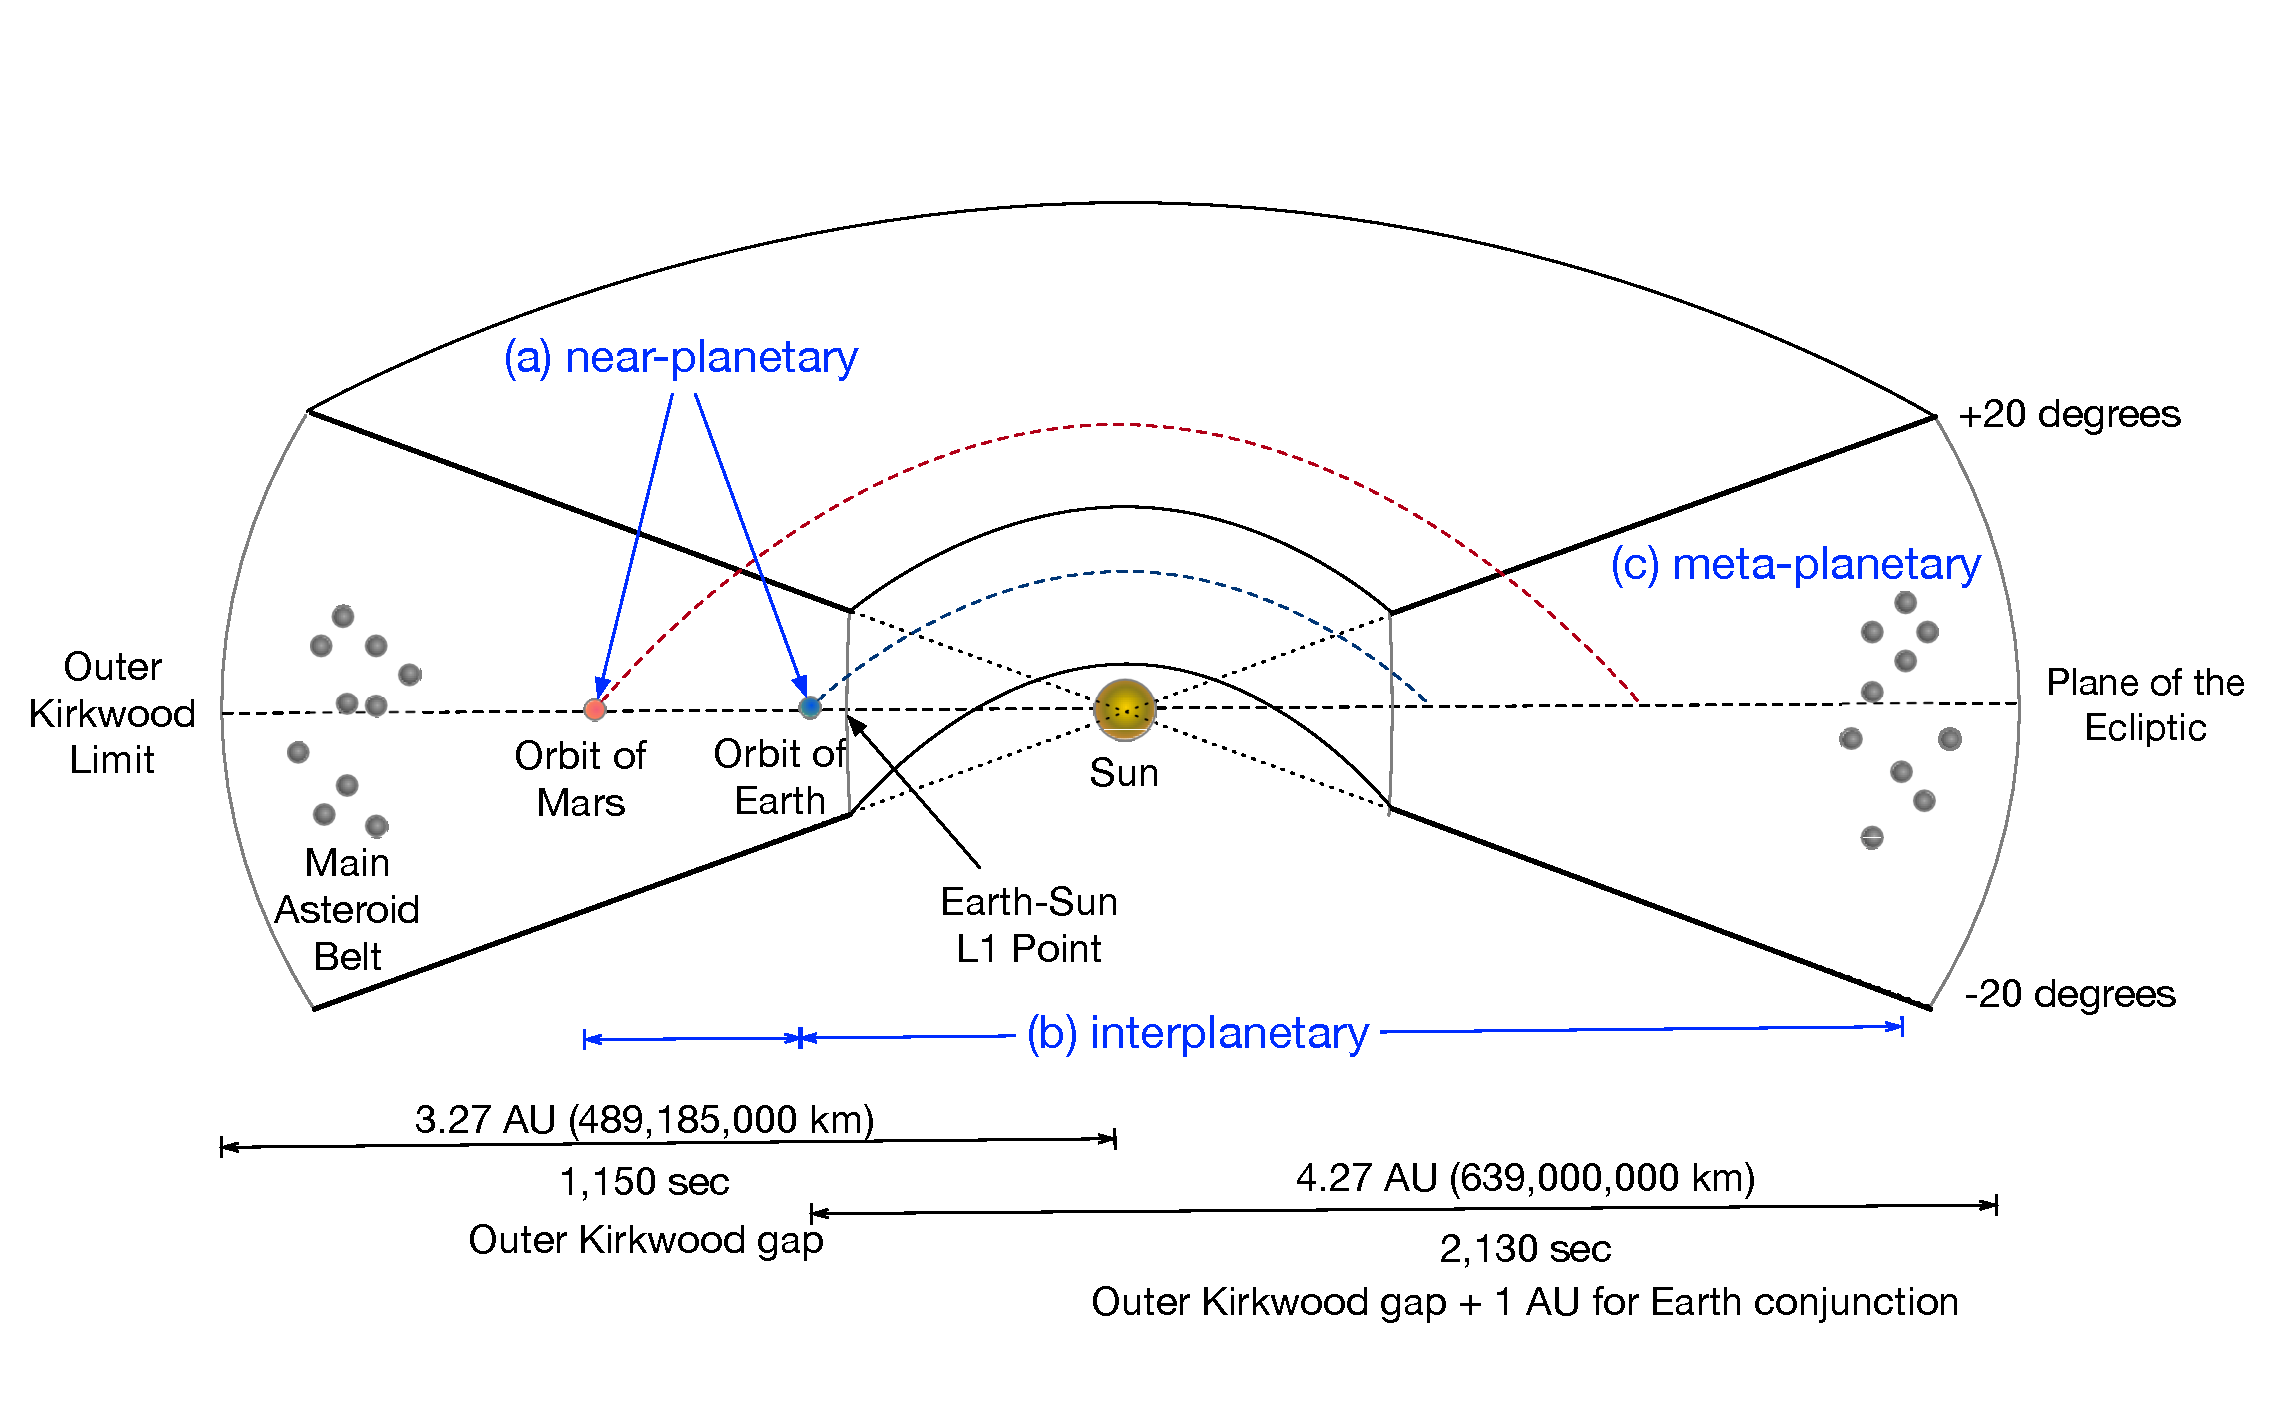
\includegraphics{figures/fig1-toroid-of-interest}
 \caption{A toroid of interest for a near-future in-space economy}
 \label{f:fig1-toroid-of-interest}
\end{figure}

Spacecraft communicating with controllers solely via relays require certain adjustments to be made to their designs to allow them to maintain fault-tolerant operations\cite{lewicki_phoenix_2006}. Those adjustments include:
\begin{itemize}
\item Provisions for autonomous operations during communications loss due to issues with the relays;
\item Control of communications rates by the relays coupled with mechanisms for automated command filtering to prevent spacecraft in a safe mode from receiving commands intended for a non-faulted spacecraft;
\item A recognition that pseudo-real-time spacecraft operational command rates will be significantly slower than direct links;
\item Designs allowing spacecraft commands to be sent ``in the blind'', with automatic handling of inappropriate commands on the spacecraft itself;
\item Designs that anticipate and automatically handle a greater number of communications disruptions due to the relays.
\end{itemize}

Some of the limitations noted above are physical and so immutable over time, such as light speed delays, and physical lines of sight. Others are dependent on the state of technology, and are thus likely to change, such as compute, memory, storage, power generation and heat rejection. Economic transactions in space are similarly most likely to start as small in message sizes, bandwidth usage, and in absolute number, but may reasonably be expected to grow by orders of magnitude as an in-space economy develops and becomes a mainstream activity. Any proposed technological solution to treat these requirements as design criteria should therefore take into account those that might change and those that are fixed.

Difficulties in communication with spacecraft have been experienced for decades, and solutions have been implemented in depth. Newer techniques have included experiments with lasers to increase the directionality, and hence the available bandwidth, of direct spacecraft communications. However, regardless of available bandwidth, the limitations above will continue to dominate communication systems. The Consultative Committee for Space Data Systems, an international cooperative body to create space data standards, has been working on this problem since the 1980s. The CCSDS File Delivery Protocol (CFDP) has provided a standard file transfer protocol for transmitting data to spacecraft since 2002\cite{CCSDS_2007}. CFDP supports both unreliable and reliable file-oriented data transfer. While these standards are increasingly comprehensive, spacecraft flight software implementations of them are almost always partial (often with cost/implementation-convenient violations of the standards), and not yet available in open-source repositories.

Data transfer over unreliable communication links can nevertheless be made reliable by the use of various error-detection and error-correction schemes. NASA's deep space missions and some commercial telecommunications satellites are currently using forward error-correction Turbo codes\cite{berrou_near_1993} for this purpose.  Data security considerations for deep space missions has thus far been minimal, as the physical barriers to interacting with these assets are severe.

A useful approach to abstract above current Internet networking protocols for an ``interplanetary Internet'' was developed to ensure delivery of file-oriented data in a ``postal model of communication''\cite{burleigh_delay-tolerant_2003}. This email-like functionality over communications systems with very high degrees of transmission latency was specifically aimed at deep space communications challenges. The effort was confusingly known as Disruption Tolerant Networking at the funding agency, the U.S. Defense Advanced Projects Research Agency (DARPA). Unfortunately, the proposals did not progress to the Standards Track of the Internet Engineering Task Force where they were originally published, and the original research group disbanded around 2005. New work on Delay/Disruption Tolerant Networking currently continues at NASA\cite{mahoney_disruption_2016}.

Prototypical implementations of Delay/Disruption Tolerant Networking demonstrated successful operation with delays lasting up to sixty minutes. Round-trip communication delays in the Earth-Moon-Mars-asteroid belt toroid suggest the motivating factor in testing delays of that period.

The notional ``heart'' of a blockchain is its consensus algorithm. A blockchain consensus algorithm defines the steps necessary for blockchain participants to agree on information to be added to the distributed ledger. It is how the nodes in the network agree (come to consensus on) the next block to be added to the chain\cite{hyland-wood_future_2018}.

Existing blockchain consensus algorithms have been recognized by many as limiting the applicability of blockchains to space operations\cite{yu_blockchain_2019,yu_situational_2019,mandl_bitcoin_2017,molesky_blockchain_2018,xu_exploration_2019}. It is particularly important to recognise the engineering tradeoffs inherent in increasing power consumption on spacecraft\cite{lyke_energy_2017}.

Several researchers have suggested the applicability of Ethereum as a possible blockchain framework (e.g. \cite{israel_space_2019}), but noted that the consensus algorithms currently used on the public production Ethereum blockchain (known as ``Ethereum MainNet'') are inappropriate for use in space operations\cite{molesky_blockchain_2018,xu_exploration_2019,mital_blockchain_2019}. Neither the traditional proof of work (PoW) algorithm nor the forthcoming proof of stake (PoS) consensus algorithm used on Ethereum MainNet or its public test networks provide the properties needed for space operations. For example, Ethereum PoW is intentionally designed to be computationally intensive, and Ethereum PoS relies upon the blockchain having an economically meaningful cryptocurrency to be used for internal operations. Neither algorithm would cope well with blockchain nodes operating in a significantly time-delayed, or low-availability network environment.

Changing the consensus algorithm of an Ethereum system creates a blockchain that is incompatible with Ethereum MainNet, at least under the current state of the art. Those taking this path (e.g. the Enterprise Ethereum Alliance and its members, and those researchers cited in the previous paragraph) are thus proposing ``private'' or ``enterprise'' Ethereum blockchains with consensus algorithms and perhaps other properties they deem appropriate for operations in their contexts.

Three groups have suggested the Practical Byzantine Fault Tolerance (PBFT) algorithm\cite{castro_practical_1999} as a possible consensus algorithm for near-Earth orbital space operations\cite{yu_blockchain_2019,molesky_blockchain_2018,mital_blockchain_2019}. PBFT is a so-called proof of authority (PoA) algorithm, in that certain network nodes are given authority to act as proxies for many other nodes. One presumes those researchers meant to suggest PBFT as modified for use as a blockchain consensus algorithm, e.g. Istanbul Byzantine Fault Tolerance\cite{lin_istanbul_2017}, since PBFT was not itself defined with blockchains in mind. The PBFT family of consensus applications are an imperfect fit for orbital space operations given their reliance on time and connectivity as critical algorithmic components. Timeouts resulting from communications delays, occultation, radio interference, and other communication disruptions are all too common with spacecraft, but are used to determine error conditions in the PBFT family of consensus algorithms. PBFT algorithms would be an even less perfect fit for deep space operations where such communication disruptions are routinely expected. PBFT message sizes also tend to be large in practice, which work against the bandwidth, processing, and storage capabilities of most extant and proposed spacecraft. However, blockchains using PBFT algorithms located terrestrially may still be a reasonable component of integrated space systems.

As noted by Beldavs, ``Central to the economy is money and rules for transacting business, as well as institutions that facilitate business activity such as banks.''\cite{beldavs_blockchains_2016} Blockchains can theoretically fulfill all of those criteria. The two largest, and earliest, public blockchains Bitcoin\cite{nakamoto_bitcoin_2008} and Ethereum\cite{buterin_ethereum_2013,wood_ethereum_2014} have both created usable currencies (in spite of their volatile prices), have defined rules for transacting business, and include smart contract functionality\cite{szabo_smart_1994} that may be used to facilitate business activity.

Beldavs suggests that the establishment of property rights and the use of a property registration system are necessary conditions for the establishment of an in-space economy\cite{beldavs_blockchains_2016}. He asserts that any future property rights over space resources ``will need to be compliant with the Outer Space Treaty that excludes conventional real property whose ownership rights are granted by a sovereign state.'' While he is correct in quoting Article II of the Outer Space Treaty\cite{UNCPUOS_1967} ``Outer space, including the moon and other celestial bodies, is not subject to national appropriation by claim of sovereignty, by means of use or occupation, or by any other means'', it is currently unclear that the Outer Space Treaty will survive large-scale economic activities in space, nor that those with fortunes to be made will voluntarily bind themselves to it. The approach generally taken in the field of economics, i.e. empirically considering the choices humans make given incentives, would tend to indicate that exactly the opposite may happen. The Outer Space Treaty is likely to be replaced by subsequent agreements that both allow and foster an in-space economy. Others have noted that the current legislative structures focus on ``the non-militarisation of space, the promotion of scientific endeavours and the mitigation of orbital debris. However, the legislative framework does not presently anticipate the use of orbital planes in LEO for commercial actors or the management of orbital shells for LEO.''\cite{green_mitigation_2018} Effective ``natural monopolies'' could therefore form (in the absence of new legislation or treaties) by commercial dominance of particularly useful orbital shells. The anticipated dominance of at least one orbital shell by SpaceX Starlink communications satellites is a topical example of such an effective monopoly, and a practical reason to suggest that the current legislation environment is unstable due to the rise of commercial space interests.

Israel has proposed that a lex mercatoria-like system similar to the economies that developed between companies operating away from their home countries during the Age of Exploration may form in space\cite{israel_space_2019}. Blockchains, with their decadal history of performing lex mercatoria-like operations, seem to be a reasonable fit for the likely conditions.


%%%%%%%%
% SECTION %
%%%%%%%%
\section{Desired Blockchain Properties}\label{sec:desiredproperties}

\textbf{TODO}: Add a brief review of blockchain consensus algorithm families and key differentiators in a space context. Introduce the acronyms (e.g. PoW, PoS, PoA) so they may be used later. Pull from ICSSC paper.

\textbf{TODO}: Introduce the considerations required related to absolute time-knowledge.  Earth-wide time synchronization to sub-millisecond timing has become trivial owing to internet time-server and GPS signals, but these facilities are not currently available in deep space, and are challenged by non-realtime communications, and offline device clock-drift at endpoints.

Several logical blockchain-spacecraft relationships are possible, and each relationship implies a different overall systems architecture. Figure \ref{f:fig2-blockchain-arch} illustrates the four possible architectural relationships between a blockchain and a spacecraft. A spacecraft may act as a regular blockchain node (a), or as a mining node, sometimes also known as a writer or a valdidator (b). A spacecraft may simply read information from a blockchain (c) or request transactions be written to a blockchain (d). These possible relationships imply very different computation capacity and radio bandwidth onboard spacecraft, especially due to overall message traffic and average message size. We will suggest a blockchain-spacecraft relationship suitable for each of the target domains.

\begin{figure}[htb]% order of placement preference: here, top, bottom
 \centering{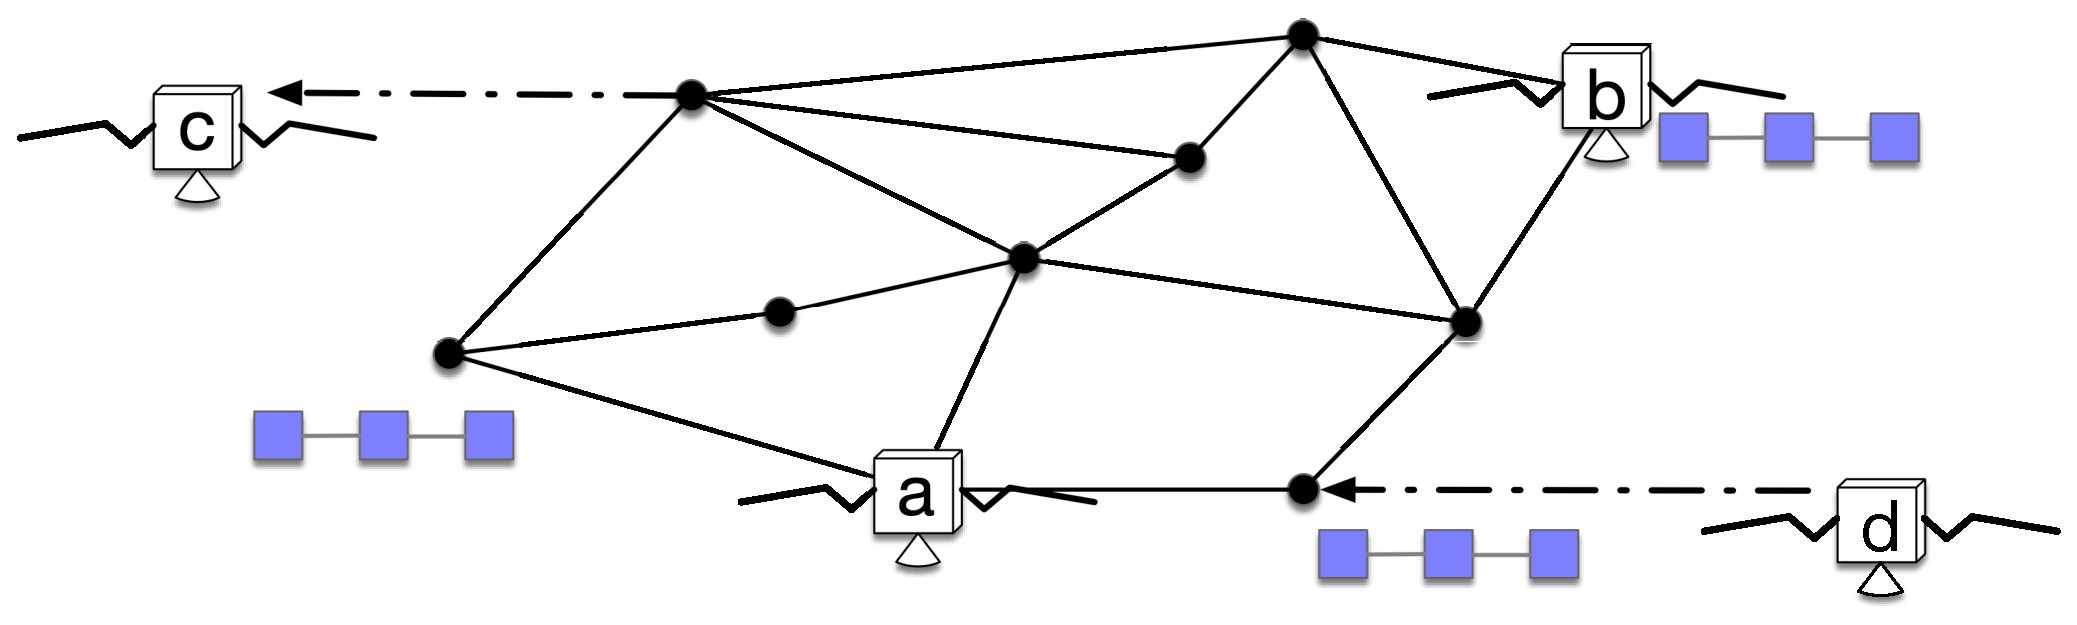
\includegraphics[width=400px,keepaspectratio]{figures/blockchain-arch}} 
 \caption{Possible blockchain-spacecraft relationships}
 \label{f:fig2-blockchain-arch}
\end{figure}

Table \ref{t:tab1-spacecraft-rels} compares the possible relationships between spacecraft and blockchains in terms of the amount of message traffic necessary to participate in each manner, and the degree to which onboard software would need to change to support blockchain operations of each type. By far the most compelling relationship between a spacecraft and a terrestrial blockchain is for the spacecraft to read information from the blockchain, as illustrated in Fig. \ref{f:fig2-blockchain-arch}(c) and compared in Table \ref{t:tab1-spacecraft-rels}. The costs for such read operations are minimal in terms of both message traffic and the degree of software changes. We therefore focused on the evaluation of technical solutions in which Earth-orbiting satellites would act as edge devices for terrestrial blockchains, with a read-only relationship.

\begin{center}
\begin{table}
\caption{Comparison of possible blockchain-spacecraft relationships}
 \label{t:tab1-spacecraft-rels}
\begin{center}
\begin{tabular}{lll}
\hline
Relationship    & Message traffic to/from satellite & Changes needed to onboard software \\
\hline
(a) Regular node      & High    & High      \\
(b) Mining node       & High     & High      \\
(c) Read-only       & Low     & Low-Medium      \\
(d) Write request & Low      & Medium       \\
\hline
\end{tabular}
\end{center}
\end{table}
\end{center}


\subsection{Near-Planetary Economies}

\textbf{TODO}: Blockchain properties for operations within the orbits of an outer moon (e.g. cislunar and cisdeimotic space).

\subsubsection{Consensus Algorithm Selection for Near-Planetary Space}

\textbf{TODO}: Primarily from the ICSSC 2019 conference paper.

As noted in the literature review, three groups have suggested the Practical Byzantine Fault Tolerance (PBFT) algorithm as a possible consensus algorithm for near-Earth orbital space system operations. 

\textbf{TODO}: Describe Table 2

\begin{center}
\begin{table}
\caption{Proof of Authority Consensus Algorithms with Immediate Finality}
 \label{t:tab2-poa-algos}
\begin{center}
\begin{tabular}{llll}
\hline
Algorithm    & Message traffic to reach consensus & Average message size & Resilience to lost messages \\
\hline
Honey Badger      & O($n^{2}$)    & O(b)   & No   \\
Tendermint       & O($n^{2}$)     & O(b)  & No      \\
DBFT       & O($n^{2}$)     & O(b)  & No      \\
IBFT 2.0 & O($n^{2}$)      & O(b)  & Yes       \\
\hline
\end{tabular}
\end{center}
\end{table}
\end{center}


\subsection{Interplanetary Economies}

\textbf{TODO}: Blockchain properties for interplanetary crosschain operations (e.g. Earth-Mars).

\textbf{TODO}: Cite crosschain work.

\subsubsection{Consensus Algorithm Selection for Interplanetary Space}

\textbf{TODO}: Primarily from \href{https://docs.google.com/document/d/16O1zB_lcD3egKadkRsFOPac2bynLB9gTbNVr9kFf3HA/edit}{Consensus Algorithm for an In-Space Economy} and \href{https://docs.google.com/document/d/1rzcag5pdtEJBVtK_JrG3c8htZkn-xGRbSOg5MPRNL3s/edit}{Algorithm Evaluation for Blockchains in Space}


\subsection{Local Autonomy in Metaplanetary Space}

\textbf{TODO}: Asynchronous protocol for lex mercatoria operations between spacecraft.

\subsubsection{Consensus Algorithm Selection for Metaplanetary Space}

\textbf{TODO}: Primarily from \href{https://docs.google.com/document/d/16O1zB_lcD3egKadkRsFOPac2bynLB9gTbNVr9kFf3HA/edit}{Consensus Algorithm for an In-Space Economy} and \href{https://docs.google.com/document/d/1rzcag5pdtEJBVtK_JrG3c8htZkn-xGRbSOg5MPRNL3s/edit}{Algorithm Evaluation for Blockchains in Space}


%%%%%%%%
% SECTION %
%%%%%%%%
\section{Evaluation}\label{sec:evaluation}

\textbf{TODO}: Reporting on performance limitations would be good (e.g. message traffic as a function of consensus formation).


%%%%%%%%
% SECTION %
%%%%%%%%
\section{Conclusions}

TODO


%%%%%%%%
% SECTION %
%%%%%%%%
\section{Further Work}

TODO:
\begin{itemize}
	\item{Immediate next steps}
	\begin{itemize}
		\item Note the concept of blockchain is changing rapidly. More generalised blockDAG /transaction DAG approaches should be considered as they develop to determine applicability to space domains.
	\end{itemize}
	\item{Future Research}
	\begin{itemize}
		\item more formal proofs of consensus protocols;
		\item more work on consensus for asynchronous networks and blockDAGs;
		\item more work on consensus-less protocols;
		\item more work on crosschain protocols;
		\item greater understanding of economic theories of money especially possible relationships between government regulations/policies/laws/fiat currencies and decentralised cryptocurrencies/tokenised assets;
		\item more work on the intersection of this work with changes to space law.
	\end{itemize}
\end{itemize}


%%%%%%%%
% SECTION %
%%%%%%%%
\section*{Acknowledgments}

The authors gratefully acknowledge ConsenSys AG for supporting this research, especially its PegaSys division.


\bibliography{blockchainsinspace}
\bibliographystyle{aiaa}
%\begin{thebibliography}{9}% maximum number of references (for label width)
% \bibitem{rebek:82bk}
% Rebek, A., {\it Fickle Rocks}, Fink Publishing, Chesapeake, 1982.
%\end{thebibliography}

\end{document}

% $Id: template_basic.tex,v 1.5 2004/05/23 12:49:44 kleb Exp $
